A hadron can be misidentified as a photon if fragmentation processes results in mainly neutral hadrons that subsequently decay to collimated pairs of photons.
The production of \zj\ where the \PZ\ boson decays to neutrinos is a high-rate process, and it mimicks the photon plus \met\ signature if the hadrons from the jet are misidentified.

\begin{figure}[htbp]
  \centering
  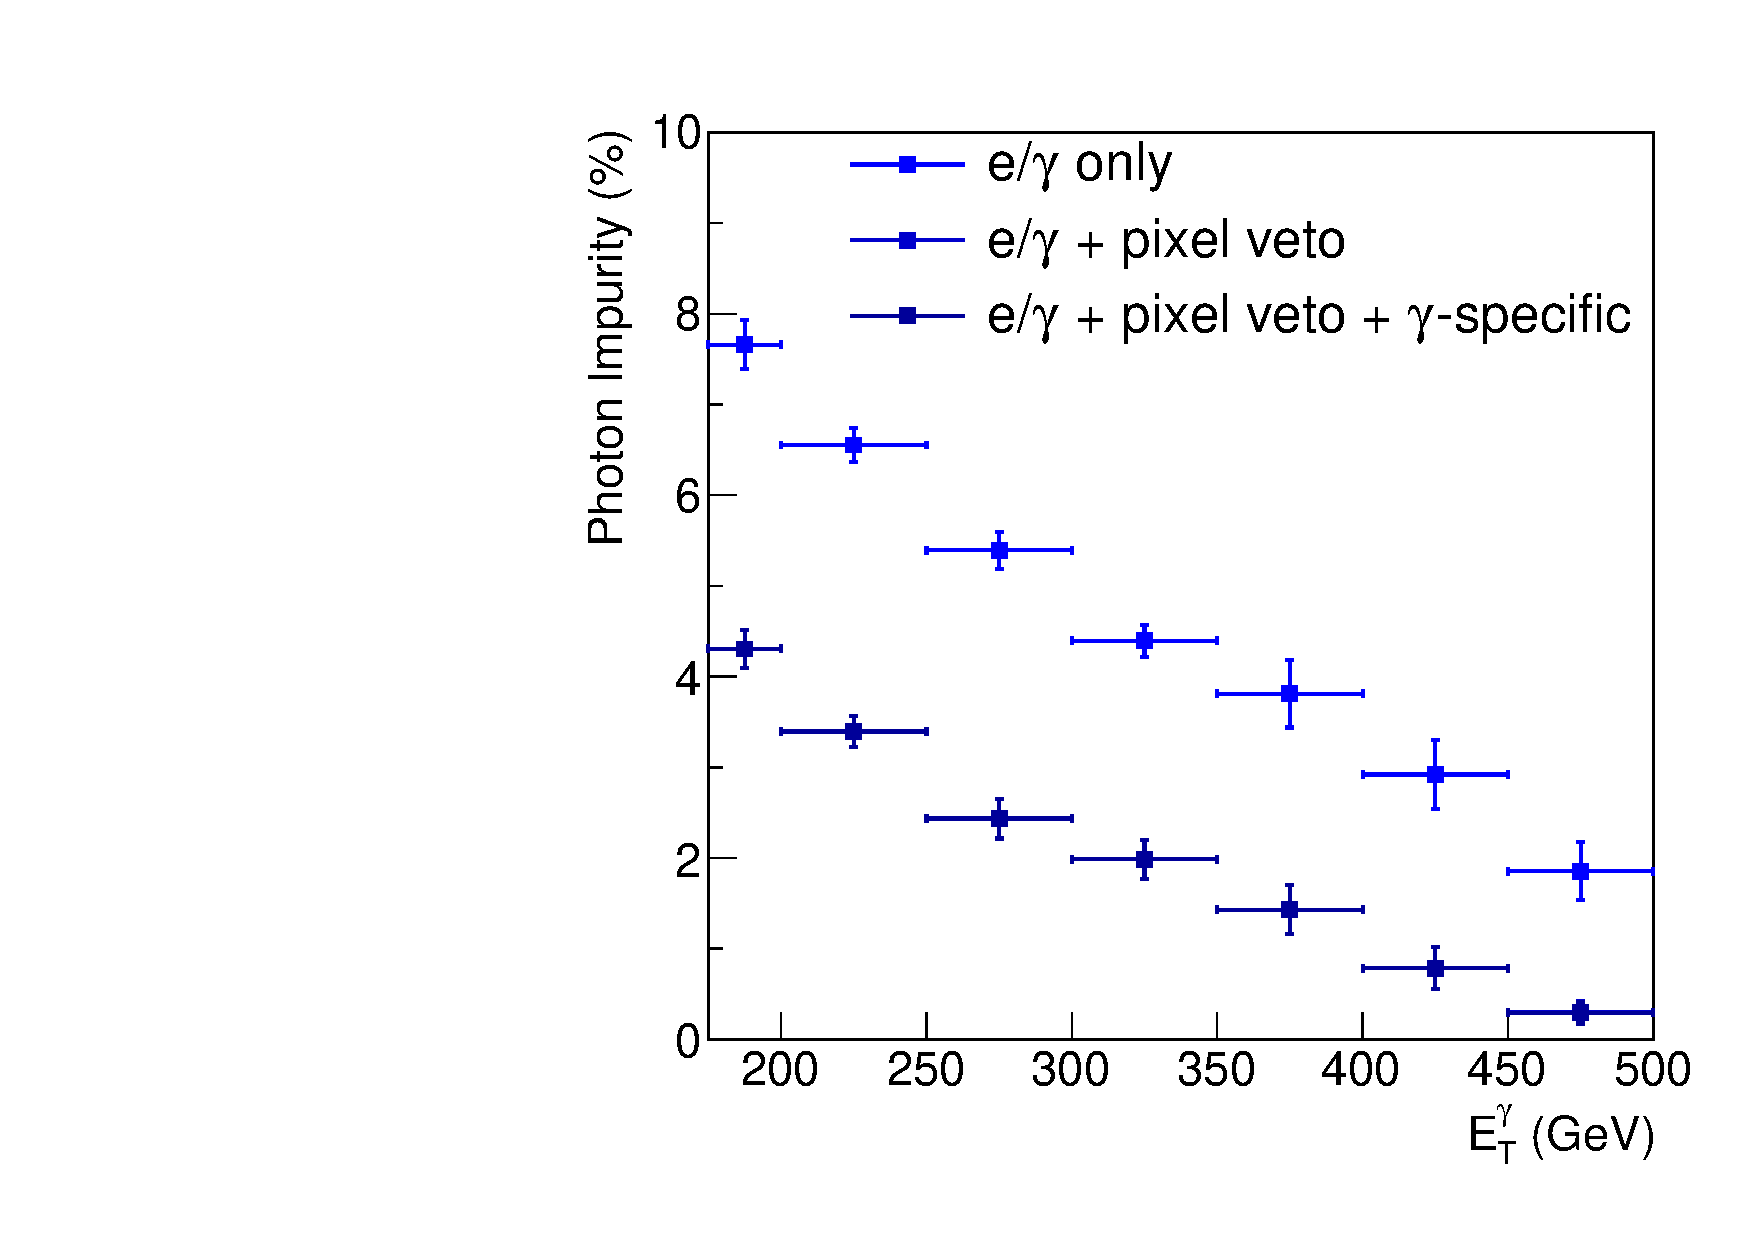
\includegraphics[width=0.49\textwidth]{Analysis/Figures/hfake/plot_impurity_barrel_medium.pdf}
    \caption{
    The percent impurity for photons as a function of \pt. 
    The different bands show the effects of adding different stages of the full ID, starting with the \egamma\ portion of the ID and successively adding the pixel seed veto followed by the rest of the \Pgg-specific portion of the ID.
    These last two curves overlap, as the non-collision rejection cuts do not effect the rate at which hadrons are misidentified as photons.
  }
  \label{fig:impurity-compsb}
\end{figure}

Without the presence of additional charged tracks or neutral hadron energy deposits, the only way to distinquish these EM-like hadrons from real photons is through the shower shape. 
Thus, we measure the fraction of hadronic objects within a pool of photon candidate objects in the EM object+jet measurement sample using the \sieie\ template fit method from Section~\ref{sec:pvsf}.
Figure~\ref{fig:impurity-compsb} and Table~\ref{tab:hfake-impurity-systs} show the final impurity and associated uncertainties as a function of \pt. 

\begin{table}[htbp]
  \centering
  \begin{tabular}{ c|c|c c c c }
    \pt & Nominal & \multicolumn{4}{ |c }{Sources of Systematic Uncertainty} \\
    (GeV) & & Sideband & CH Iso Shape & Signal Shape & Bgkd. Stats \\
    \hline
    (175, 200)  & $4.31 \pm 0.21$ & 0.09 & 0.18 & 0.05 & 0.04 \\
    (200, 250)  & $3.39 \pm 0.17$ & 0.01 & 0.16 & 0.06 & 0.03 \\
    (250, 300)  & $2.44 \pm 0.22$ & 0.14 & 0.16 & 0.06 & 0.05 \\
    (300, 350)  & $1.99 \pm 0.23$ & 0.12 & 0.16 & 0.07 & 0.08 \\
    (350, 400)  & $1.43 \pm 0.28$ & 0.23 & 0.11 & 0.05 & 0.10 \\
    (400, $\infty$)  & $0.63 \pm 0.30$ & 0.27 & 0.09 & 0.05 & 0.05 \\
  \end{tabular}
  \caption{Impurities for photons as a function of \pt.}
  \label{tab:hfake-impurity-systs}
\end{table}
  
The hadronic transfer factor $R_{h}$ measures the rate at which hadronic proxy objects result in hadrons that are misidentified as candidate photons.
The factor $R_h$ is obtained by dividing the estimated number of misidentified hadrons in the EM object+jet measurement sample by the number of events in the hadron proxy+jet measurement sample as a function of \pt. 
Figure~\ref{fig:hadronTFactor} shows the transfer factor $R_{h}$ along with the various distributions used for its derivation.

\begin{figure}[htbp]
  \begin{center}
    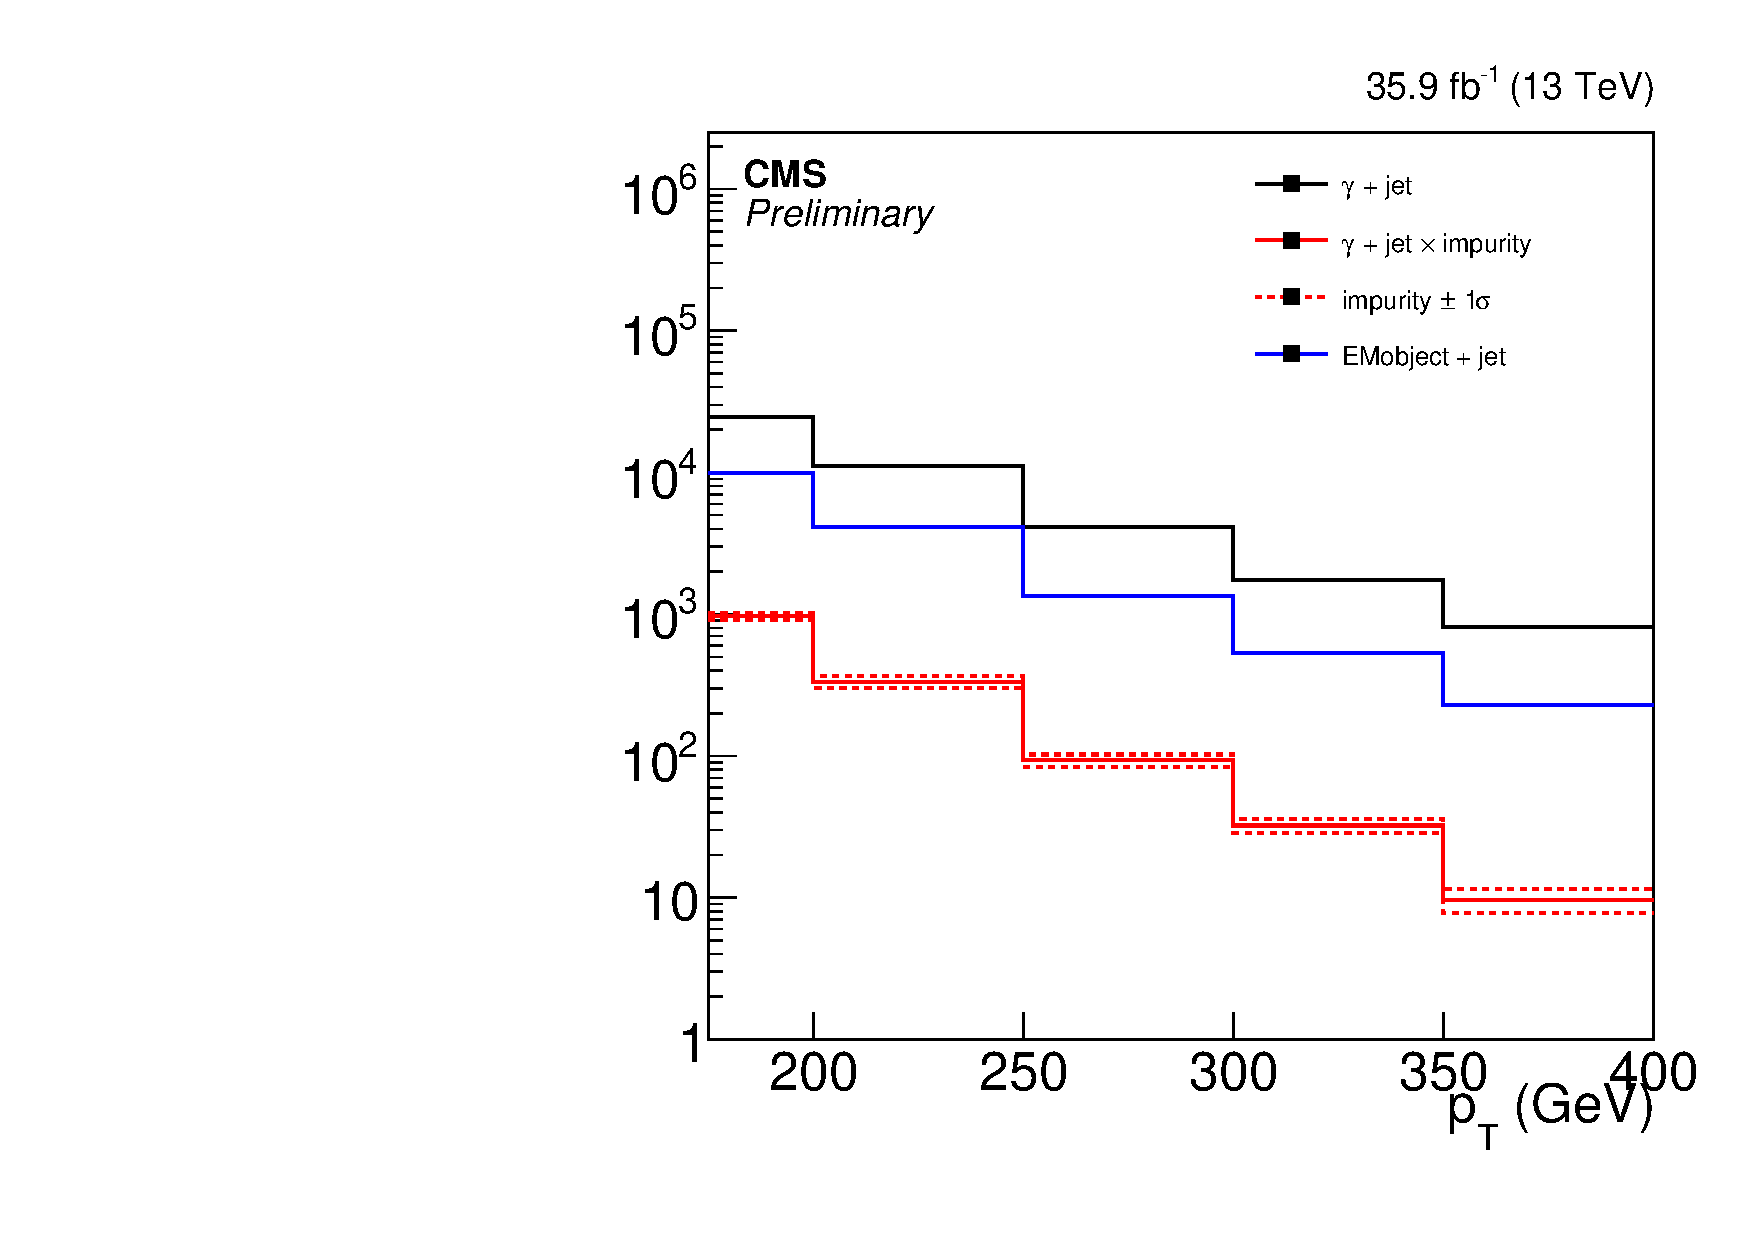
\includegraphics[width=0.45\textwidth]{Analysis/Figures/hfake/distributionsNom.pdf}
    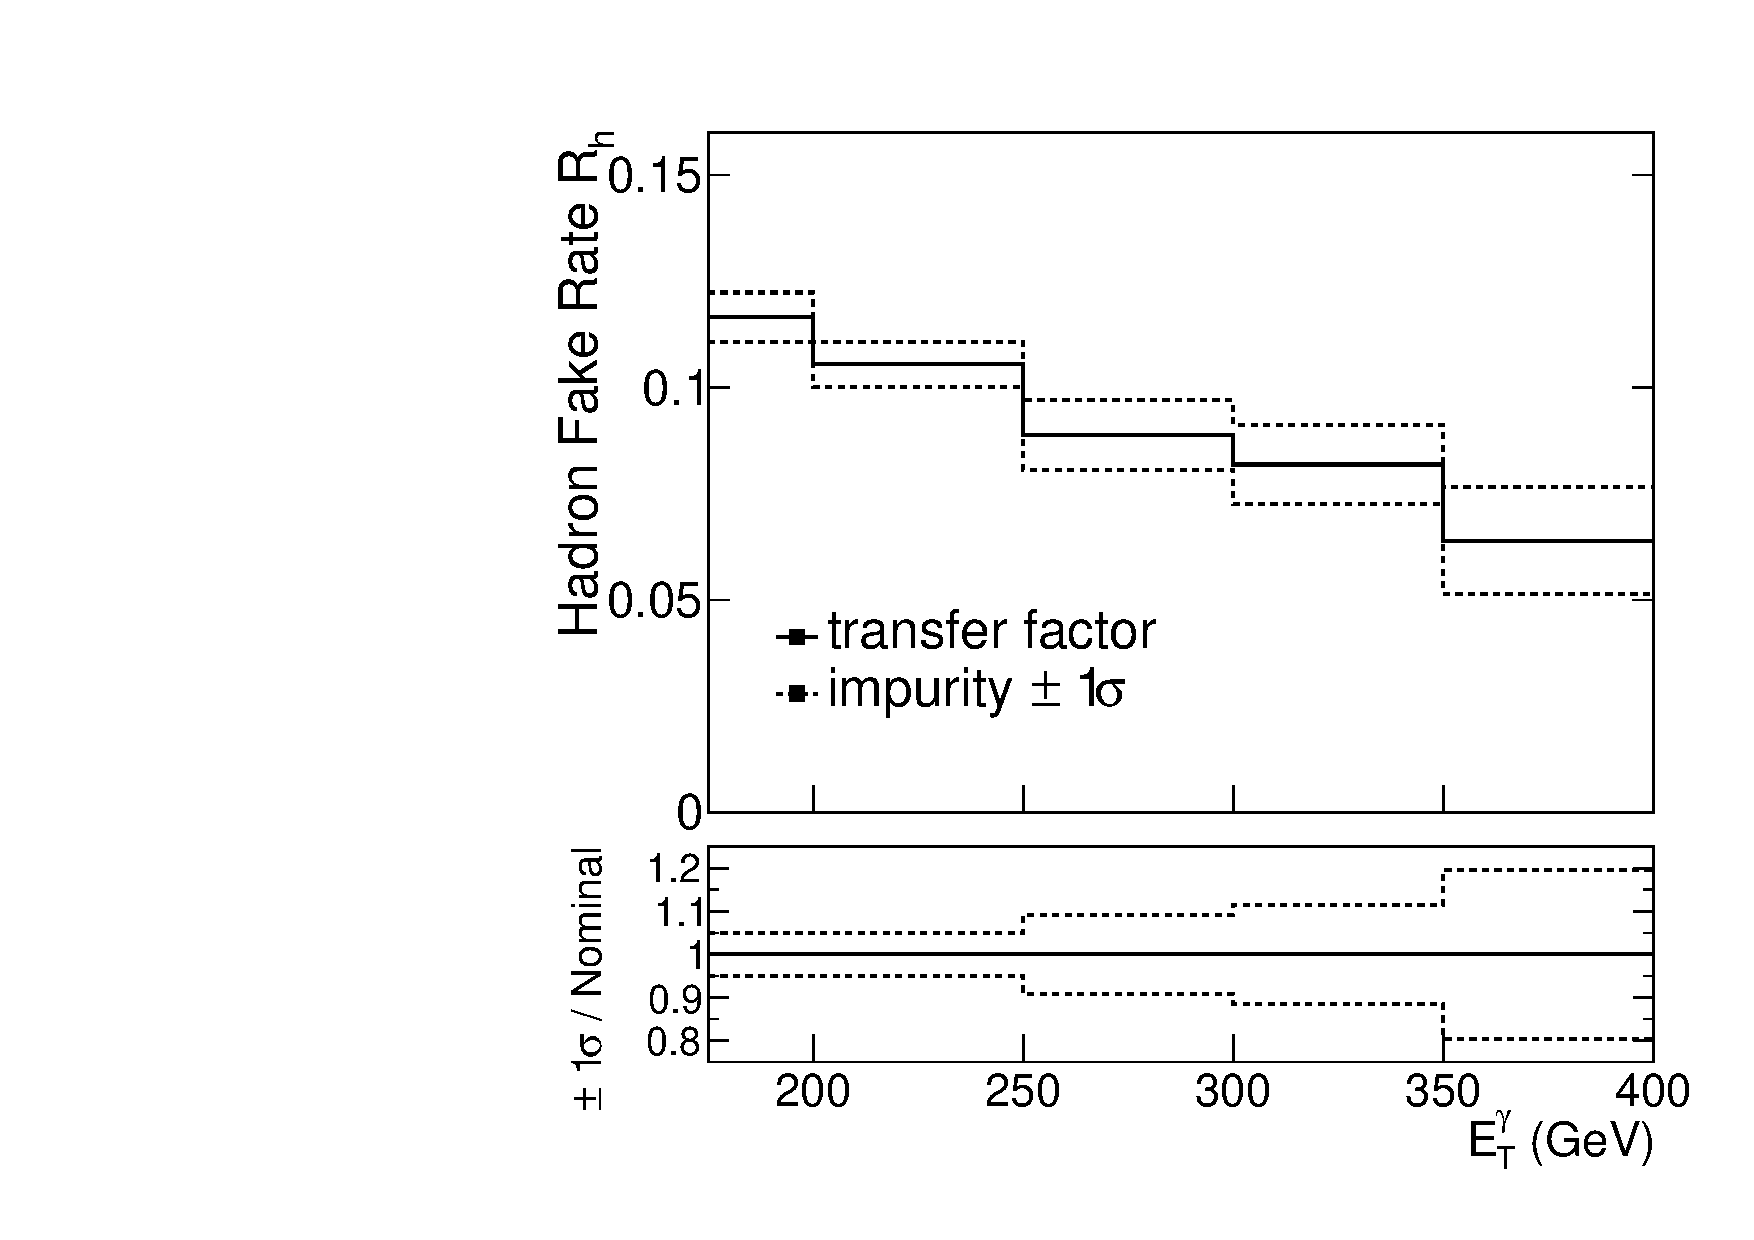
\includegraphics[width=0.45\textwidth]{Analysis/Figures/hfake/tfactorNom.pdf}
    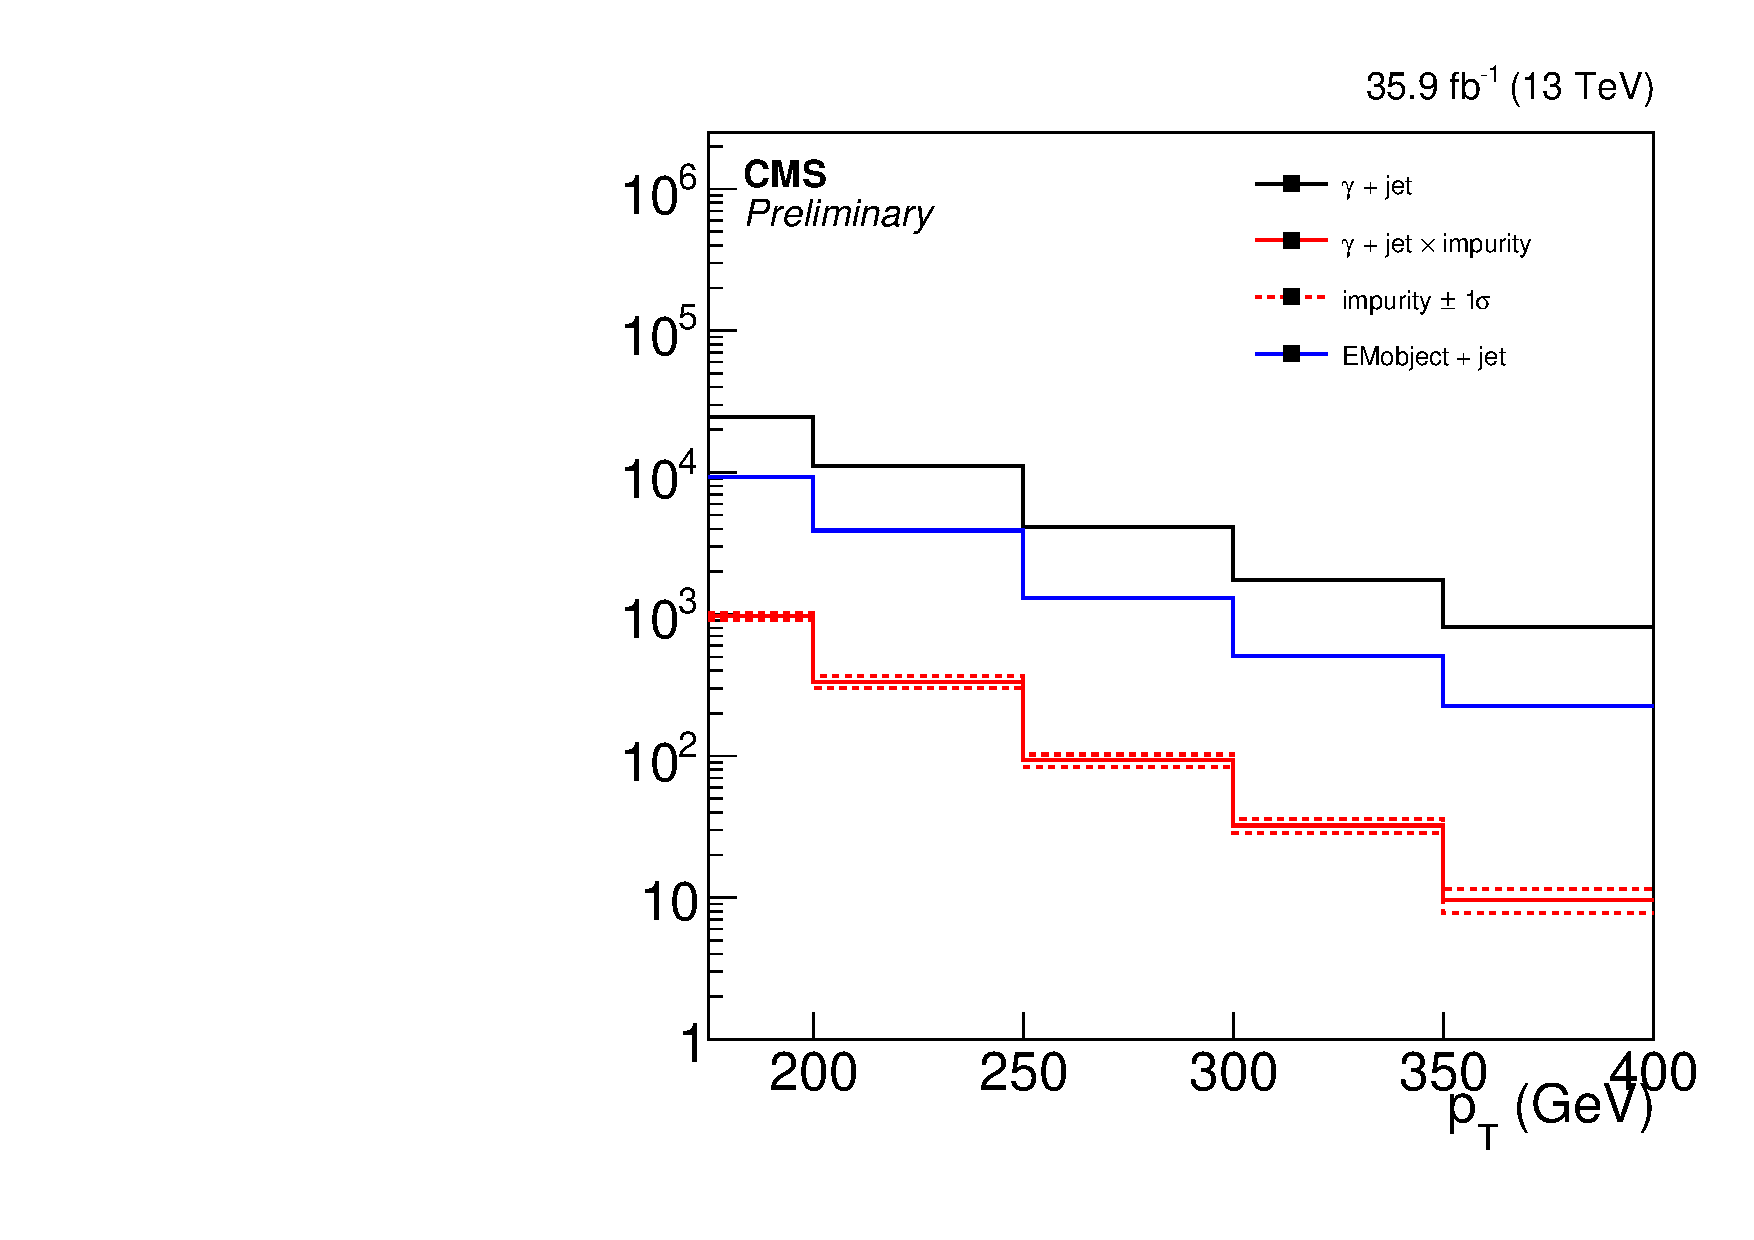
\includegraphics[width=0.45\textwidth]{Analysis/Figures/hfake/distributionsTight.pdf}
    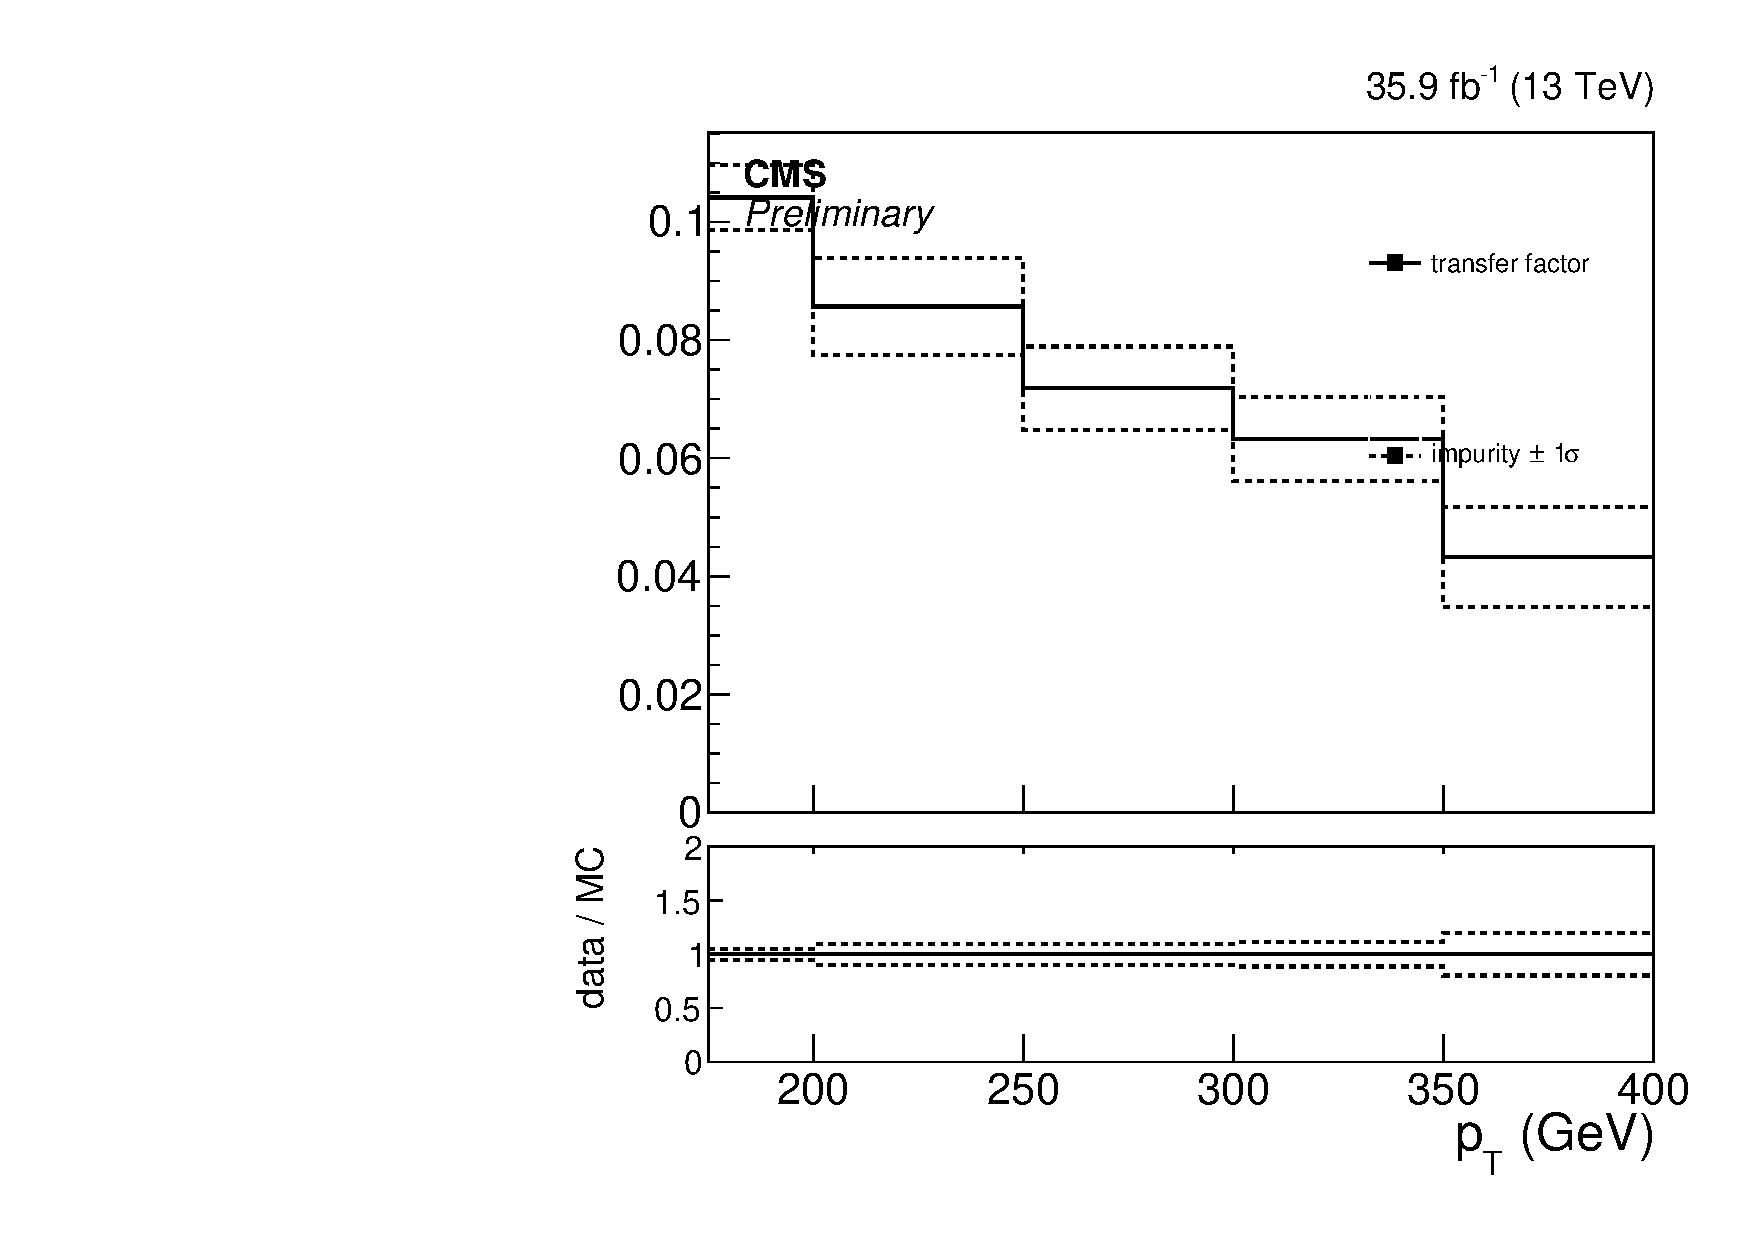
\includegraphics[width=0.45\textwidth]{Analysis/Figures/hfake/tfactorTight.pdf}
    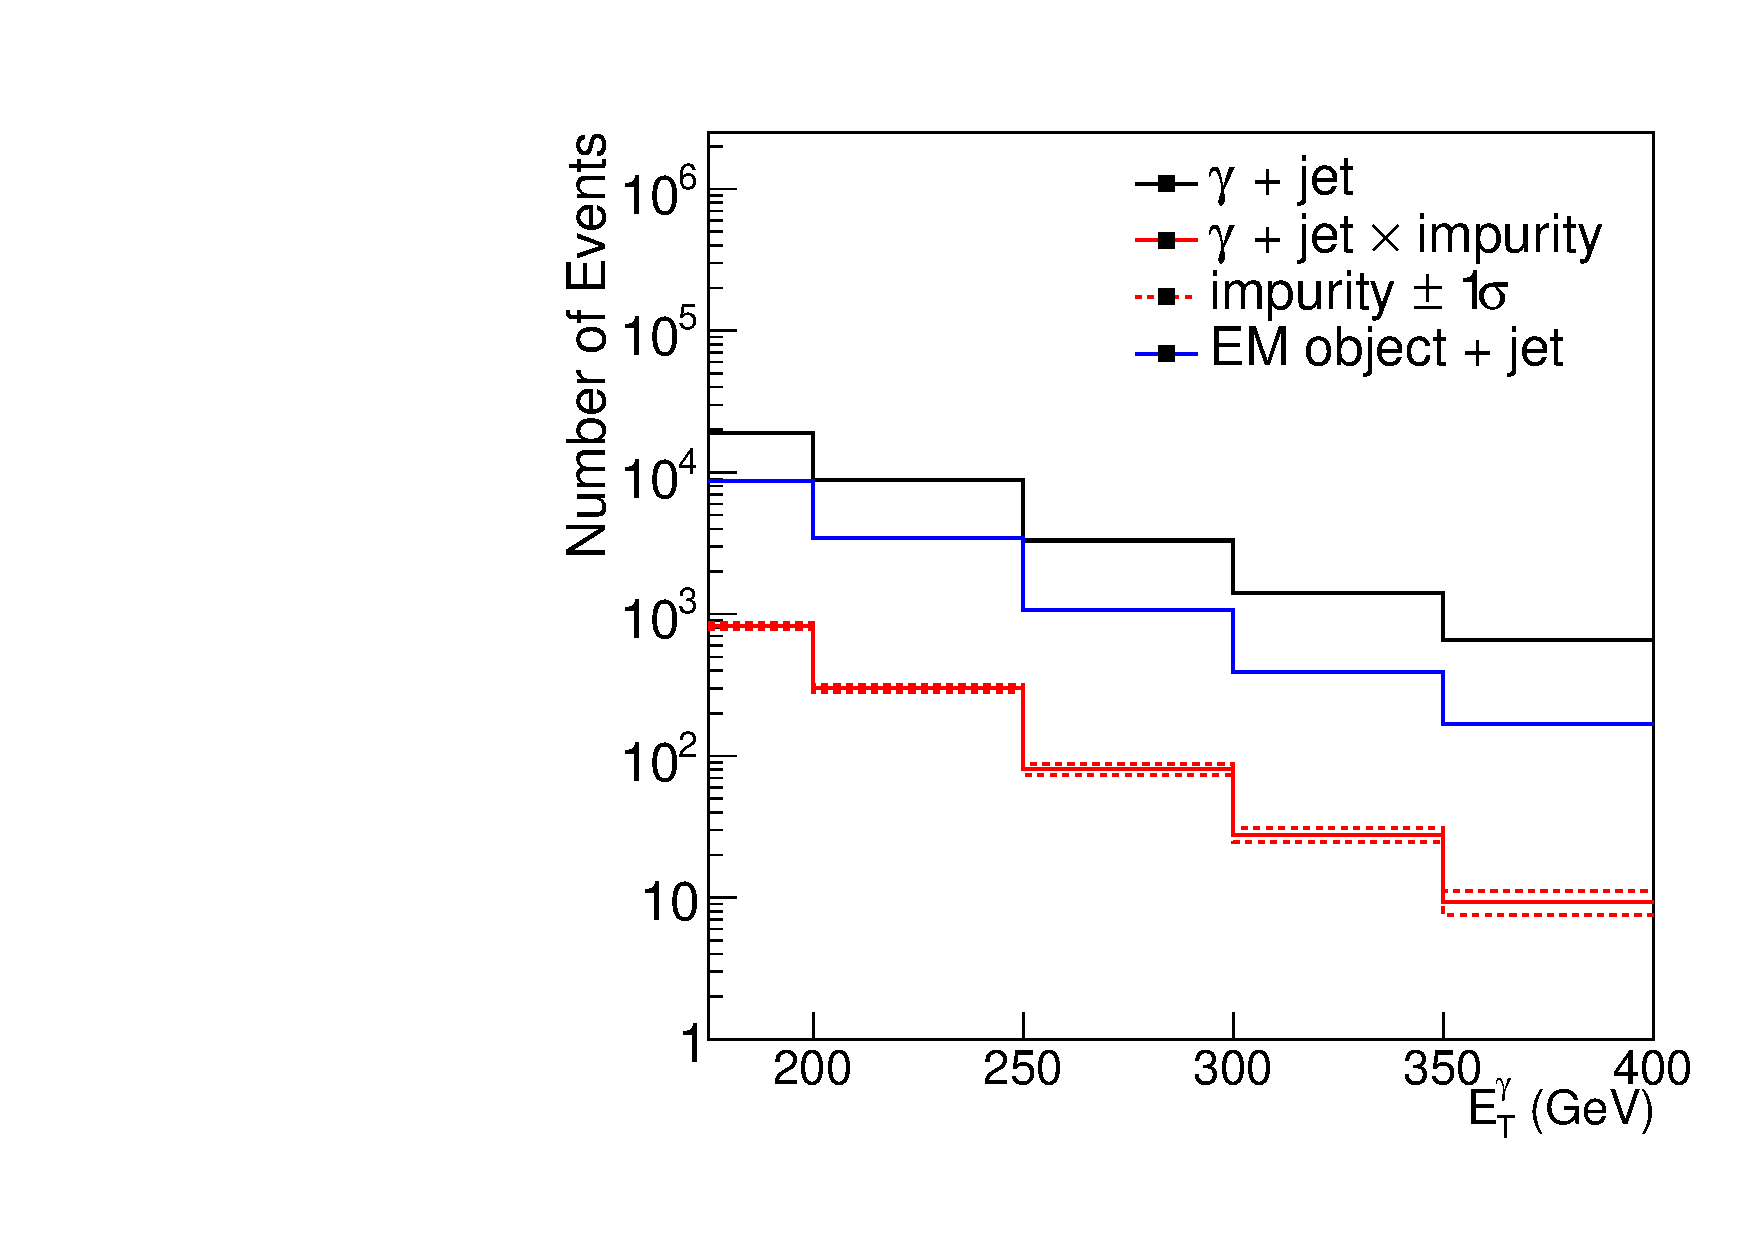
\includegraphics[width=0.45\textwidth]{Analysis/Figures/hfake/distributionsLoose.pdf}
    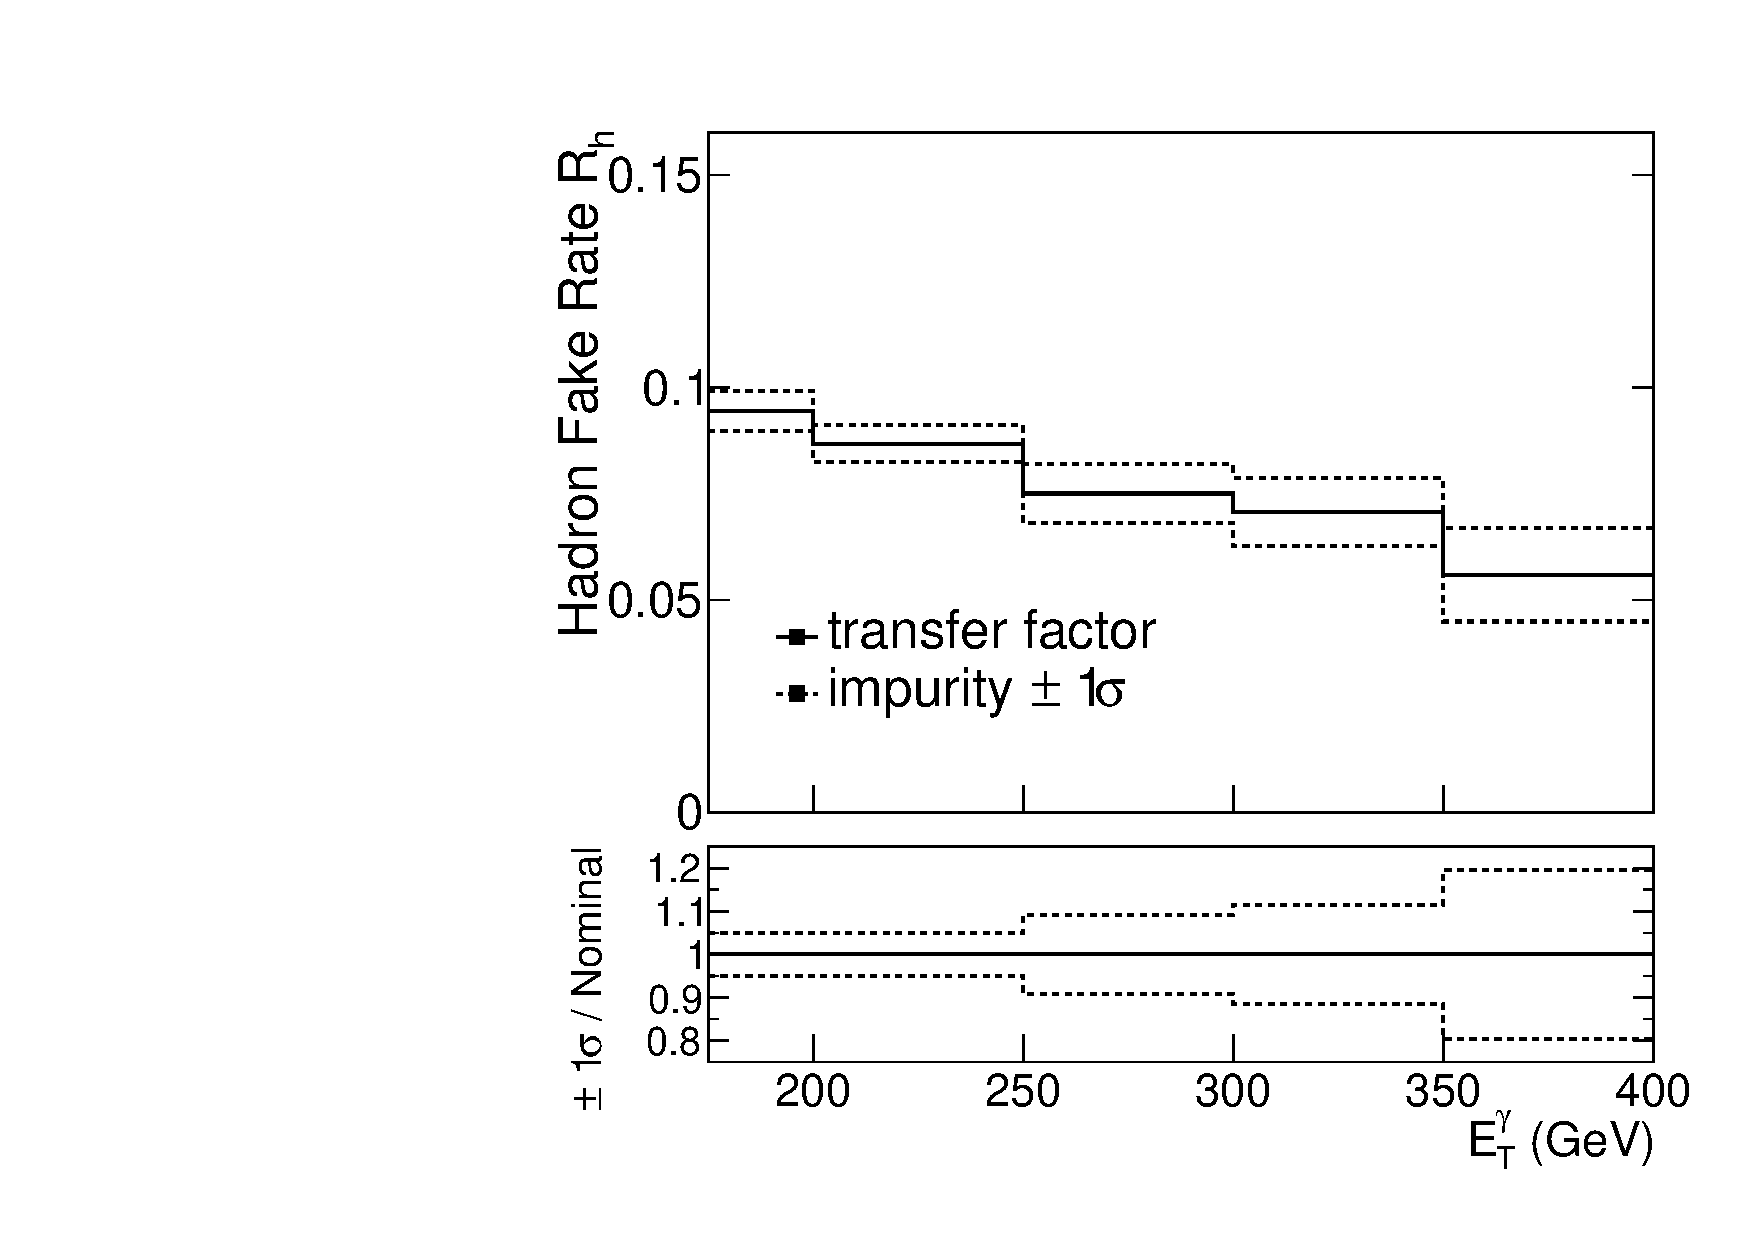
\includegraphics[width=0.45\textwidth]{Analysis/Figures/hfake/tfactorLoose.pdf}
    \caption{
      Left: The \pt\ distribution of the candidate photon object in the photon + jet control sample (black), the result of scaling it with the impurity (red), and the \pt\ distribution of the hadronic proxy object in the proxy + jet control sample (blue).
      Right: Hadronic transfer factor $R_{h}$, which is the ratio of the red and blue distributions in the left plot. 
      Top: Nominal hadron proxy object. 
      Middle: Tighter hadron proxy object. 
      Bottom: Looser hadron proxy object.
    }
    \label{fig:hadronTFactor}
  \end{center}
\end{figure}


Under the assumption that the $R_{h}$ stays constant regardless of whether the event has a high-\pt\ jet or \met, the hadron proxy sample is weighted by $R_{h}$ to determine the number of events due to misidentified hadrons in the signal region.

\begin{figure}[htbp]
  \begin{center}
    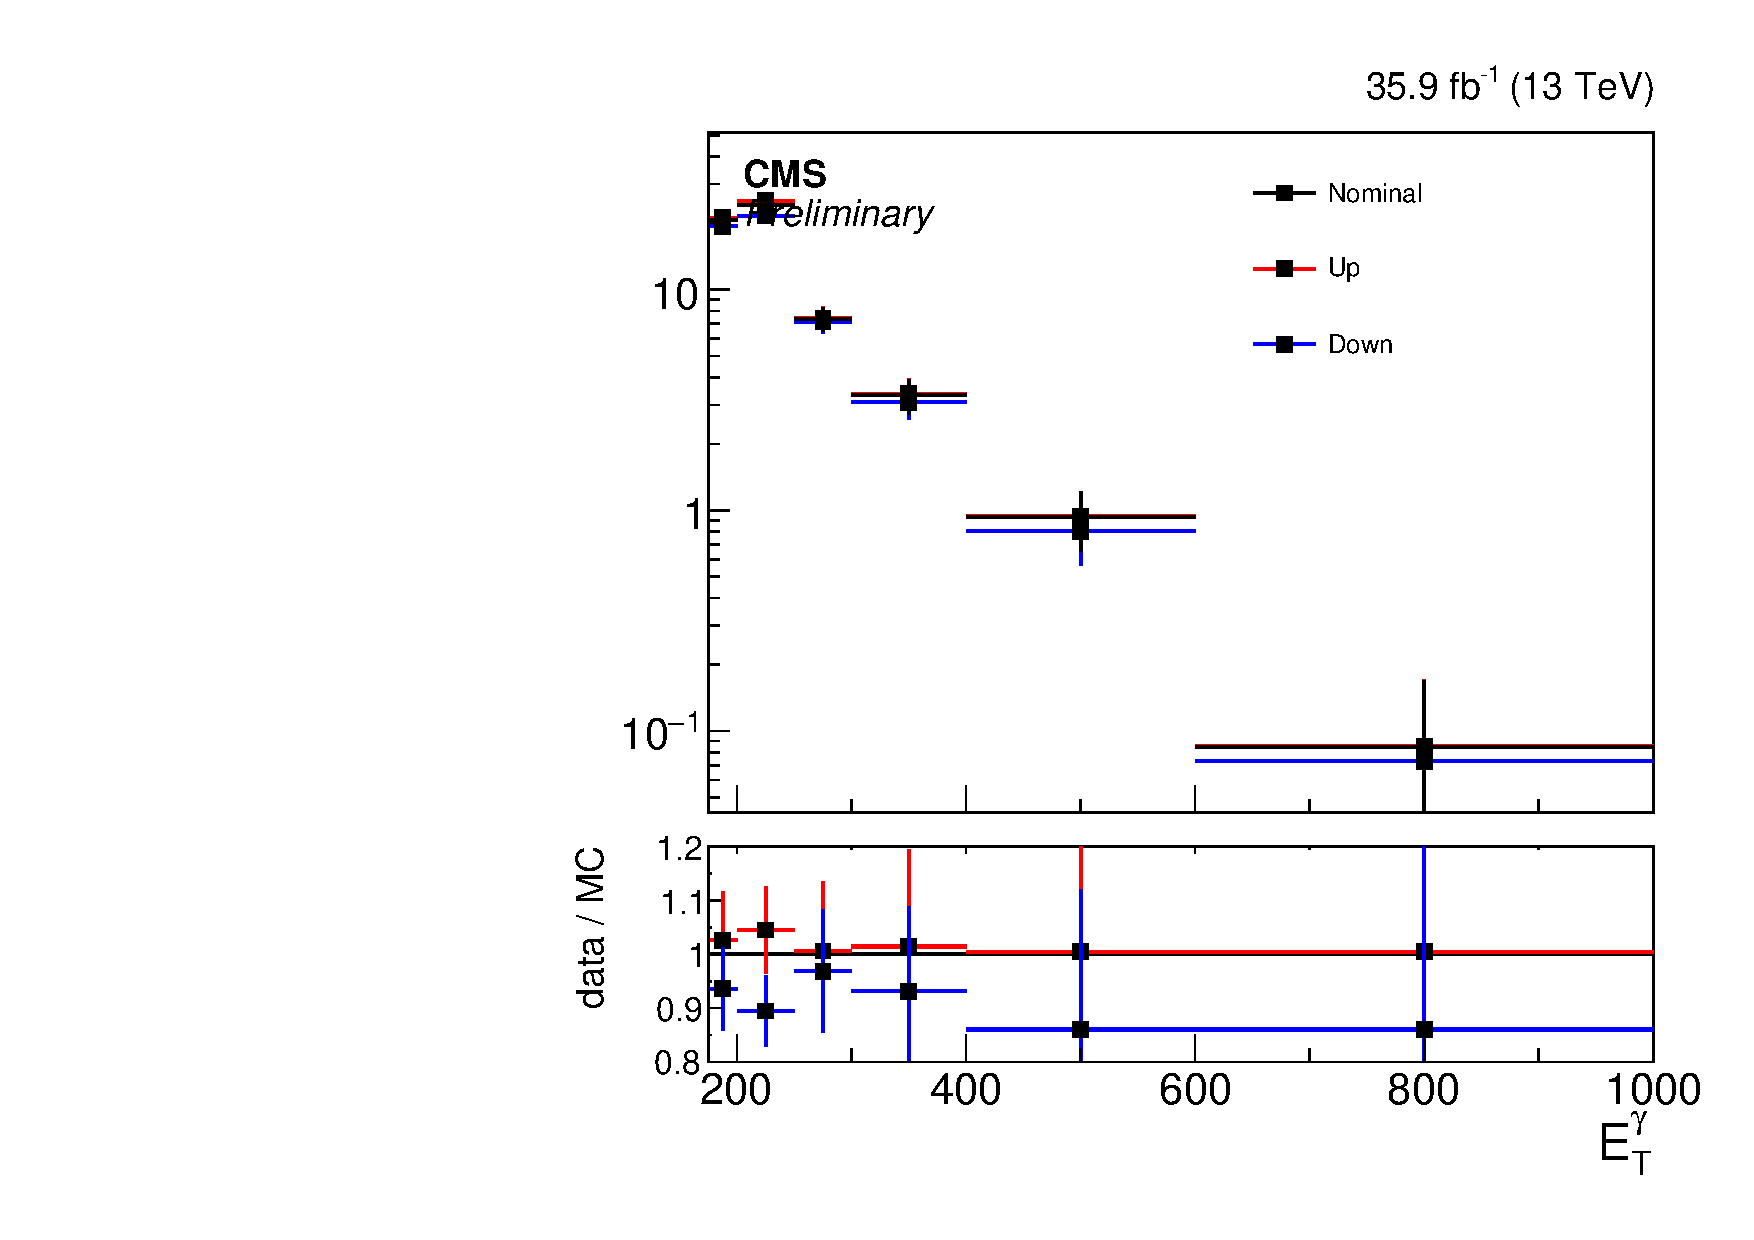
\includegraphics[width=0.49\textwidth]{Analysis/Figures/hfake/shape_sample.pdf}
    \caption{
      The \pt\ distribution of the estimated contribution from hadronic fakes in the signal region. 
      The distribution labeled Up (Down) comes from the tighter (looser) selection. 
      The systematic uncertainty resulting from this variation is around 5\% at the low end of our \pt\ range and increases to 15\% after $\pt > 400$ GeV.
    }
    \label{fig:hadronFakeShapes}
  \end{center}
\end{figure}

\begin{figure}[htbp]
  \begin{center}
    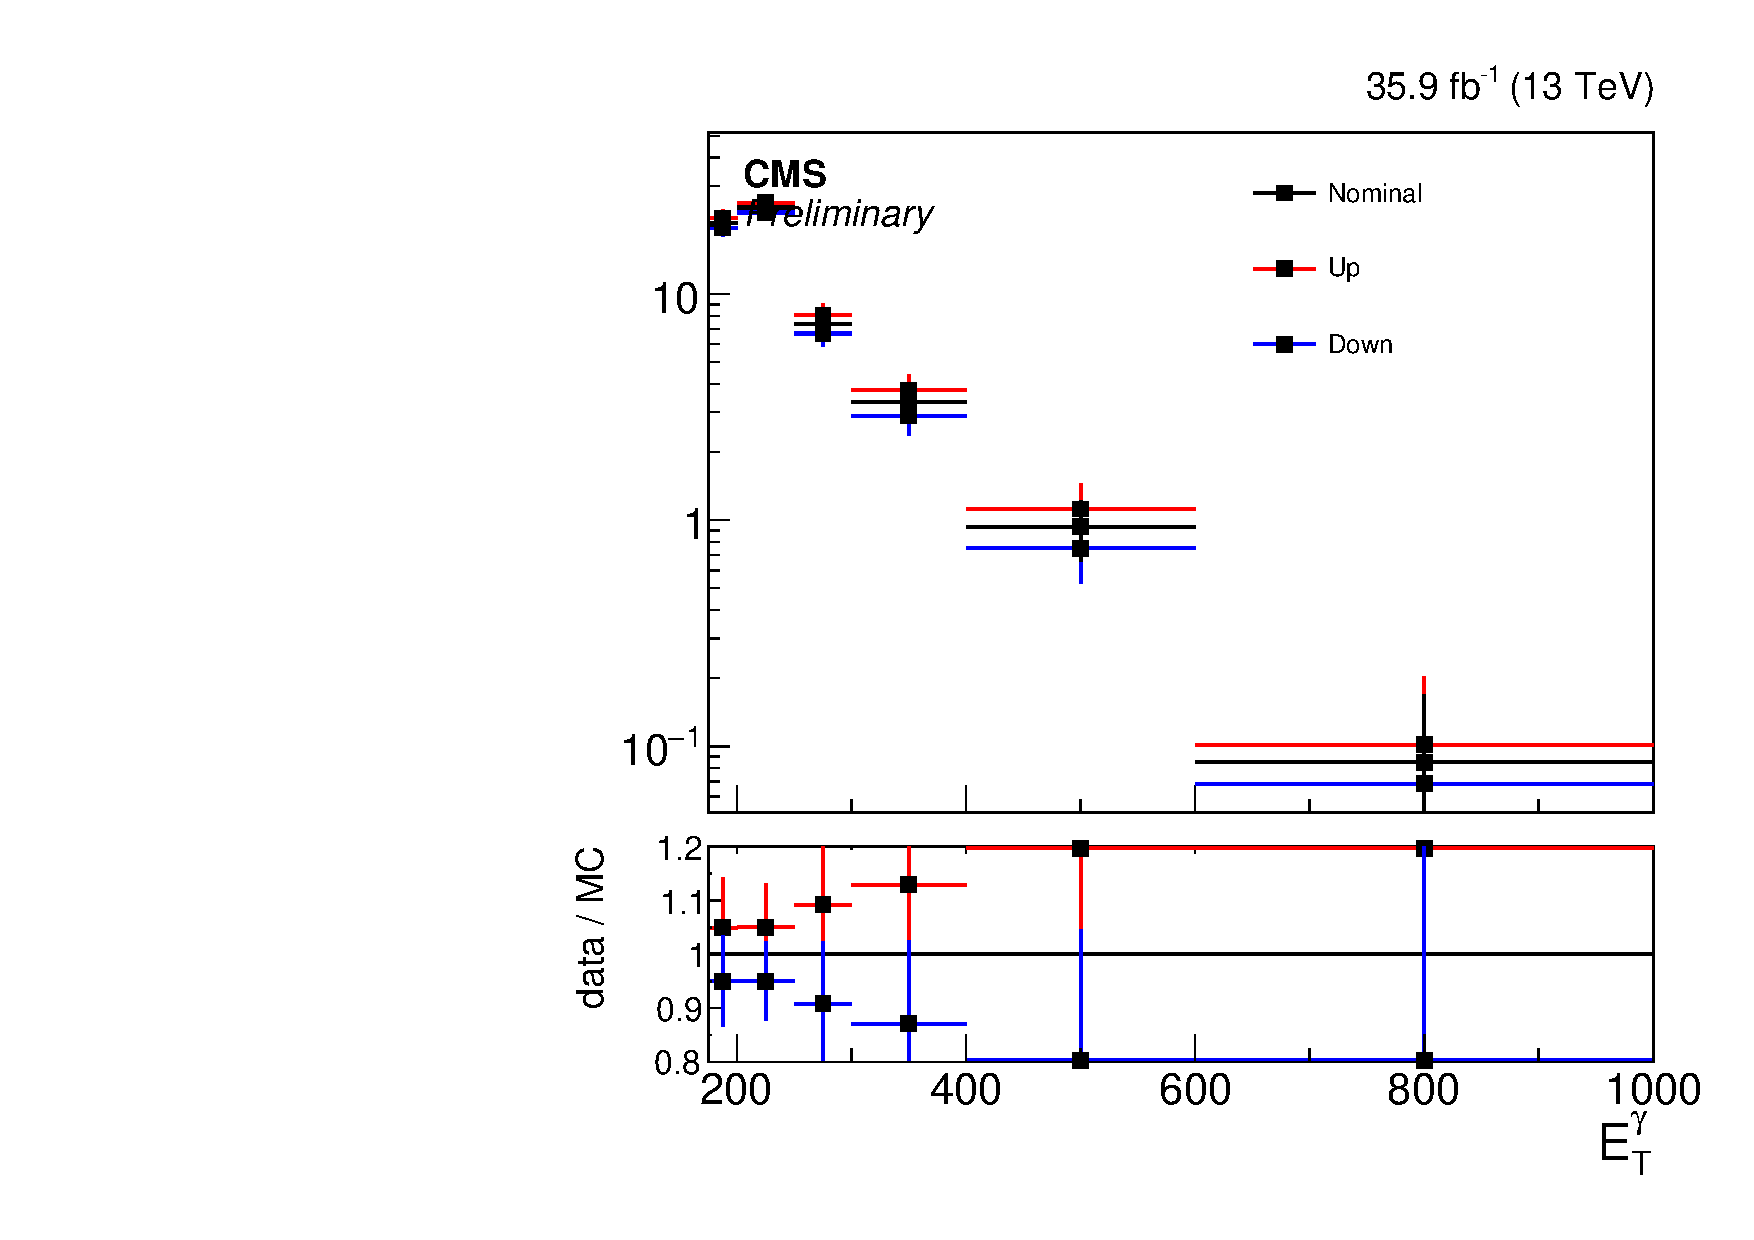
\includegraphics[width=0.49\textwidth]{Analysis/Figures/hfake/shape_purity.pdf}
    \caption{
      The \pt\ distribution of the estimated contribution from hadronic fakes in the signal region. 
      The distribution labeled Up (Down) comes from varying the purity one sigma up (down). 
      The systematic uncertainty resulting from this variation is around 5\% at the low end of the \pt\ range and increases to 20\% after $\pt > 400$ GeV.
    }
    \label{fig:hadronFakePurity}
  \end{center}
\end{figure}

To estimate the uncertainty on this background, we repeat the above method using additional proxy and measurement samples with tighter and looser definitions of the hadron proxy object.
The different distributions from the nominal, tight, and loose selections are shown in Figure~\ref{fig:hadronFakeShapes}. 
The tight and loose shapes are taken as the one sigma band around the nominal estimate. 
Additionally, there is an uncertainty coming from the estimation of the photon purity. 
Figure~\ref{fig:hadronFakePurity} shows the resulting shapes from moving the shapes generated by a one sigma shift in the purity.
